\subsection{\problemblock{*Search} Data Block}\label{sec:block-search}

Trajectories often have constraints that must be satisfied, such as a final velocity or
range. Optimization is generally used in TAOS to obtain a trajectory that meets a set
of constraints: it varies a set of parameters to maximize or minimize an objective
function subject to those constraints. If the problem is simple, however, and has only
one or two parameters and constraints, optimization may not be necessary. Because
optimization techniques are not completely reliable, TAOS provides a simpler and
more reliable search method for these cases.

\taossubhead{Search Parameters}

Each search is one-dimensional. It repeatedly changes a numerical value in the
problem file until a condition is met. For example, a constant angle of attack used to
pull out from descending flight can be varied until level flight occurs at a specified
altitude. More than one input value may be changed by one search, but every value
associated with that search is assigned the same trial value at each iteration.

Search variables are marked with the keyword \texttt{srch-n}. For example,

\begin{lstlisting}[style=taosmanual]
*fly alpha=srch-1
\end{lstlisting}

says that search 1 will determine angle of attack. The search definition itself appears
later in the problem file in a matching \problemblock{*search} block. The number in
\texttt{srch-1} relates the input location to \texttt{*search 1}. Any number of searches
may be defined, producing nested one-dimensional search loops, although problems
requiring more than two nested searches are usually better handled with optimization.

\taossubhead{Search Objective}

Every \texttt{srch-n} placeholder requires a corresponding
\problemblock{*search} block. A block for the preceding angle-of-attack example
might be

\begin{lstlisting}[style=taosmanual]
*search 1 vary alpha until alt=30000 on segment 3, trajectory 1
  xlo=0.5 xhi=10.0 xest=5.0 dx=1.0 tol=0.001
  xref=1.0 fref=10000 maxitr=20 print=1 integ=0
\end{lstlisting}

The first line defines the search objective: angle of attack is varied until altitude at
the end of segment 3 in trajectory 1 is 30,000~ft. The next two lines provide control
values. In this example angle of attack is limited to 0.5 through 10 degrees and starts
from an estimate of 5 degrees.

The parabolic methods described in \cref{sec:search-methods} vary a search value
$x$ until a search function $f(x)$ equals a specified value, reaches a minimum, or
reaches a maximum. The search function written in the data block determines which
kind of search is performed.

The first items in the block are the search number, the keyword \texttt{vary}, a name,
and the keyword \texttt{until}. The name may be any text suitable for identifying the
search parameter in the printout. The objective follows as an output variable related
to a number, another output variable, \texttt{min}, or \texttt{max}. A segment and
trajectory number are required for the first output variable, and may also be supplied
for the second. For example,

\begin{lstlisting}[style=taosmanual]
*search 1 vary pitch-rate until pitchi on segment 2
  = pitchi on segment 3, trajectory 2
\end{lstlisting}

modifies a pitch rate, most likely in a guidance rule, until the inertial pitch angles at
two segment endpoints are equal. Only one trajectory number is written, so it is
assumed to apply to both variables.

Trajectory numbers can instead be written as subscripts:

\begin{lstlisting}[style=taosmanual]
*search 1 vary weight until alt[1] on segment 3
  = alt[2] on segment 5
\end{lstlisting}

The subscript and keyword forms may not both be used for the same variable. When
segment and trajectory numbers are written with keywords, the segment number
comes first. If an endpoint number is omitted on one side of the relationship, it is
assumed to be the same as on the other side.

\taossubhead{Search Control Variables}

\Cref{tab:search-control-variables} lists the search controls. The method requires an
initial estimate \statevar{xest}, an initial increment \statevar{dx}, and lower and upper
boundaries \statevar{xlo} and \statevar{xhi}. The remaining variables have defaults
and are optional.

\begin{table}[htbp]
  \centering
  \caption{Search data-block variables.}
  \label{tab:search-control-variables}
  \small
  \begin{tabularx}{0.98\linewidth}{@{}>{\ttfamily}lX>{\ttfamily}lX@{}}
    \toprule
    \normalfont Variable & Description & \normalfont Variable & Description \\
    \midrule
    xlo & Lower search boundary & xref & Search-variable reference value (default 1.0) \\
    xhi & Upper search boundary & fref & Search-function reference value (default 1.0) \\
    xest & Initial search estimate & maxitr & Maximum number of iterations (default 20) \\
    dx & Initial search interval & integ & Search-trajectory calculation option (default 1) \\
    tol & Convergence accuracy (default $1.0\times10^{-6}$) & print & Print option (default 0) \\
    \bottomrule
  \end{tabularx}
\end{table}

The increment \statevar{dx} indicates how well the initial estimate is known. The
values \texttt{xest-dx} and \texttt{xest+dx} should bracket the solution. A small
increment implies that the estimate is close to the actual solution. The convergence
accuracy \statevar{tol} controls termination; reducing it normally requires more
iterations.

The reference factors \statevar{xref} and \statevar{fref} should make
$|x/x_{\mathrm{ref}}|$ and $|f(x)/f_{\mathrm{ref}}|$ lie between about 1 and 10. In
the first example, angle of attack ranges from 0.5 to 10 degrees, so
\texttt{xref=1.0} is suitable. The final altitude approaches 30,000~ft, so
\texttt{fref=10000} scales the search function to the desired range.

The variable \statevar{maxitr} is the maximum number of search attempts. With
\texttt{maxitr=0}, TAOS calculates only the trajectory for the initial estimate. The
\statevar{integ} variable controls trajectory recomputation. A value of one recomputes
every trajectory in the search loop and is the safer choice; zero recomputes only the
search trajectory and may be much faster. The \statevar{print} option controls
trajectory printout: zero prints only a search summary, while one prints every
trajectory generated by the search. Because the latter produces a large amount of
output, it should be used only when a search loop is being diagnosed.

\taossubhead{Search Loops}

A search starts at the beginning of the first segment containing one of its parameters
and extends to the segment specified by the objective. That part of the trajectory is
recomputed on every search iteration.

Multiple searches may be independent, as in the left diagram of
\cref{fig:multiple-search-structures}, or one may be entirely nested inside another,
as in the middle diagram. Search loops may not partially intersect, as shown on the
right.

\begin{figure}[htbp]
  \centering
  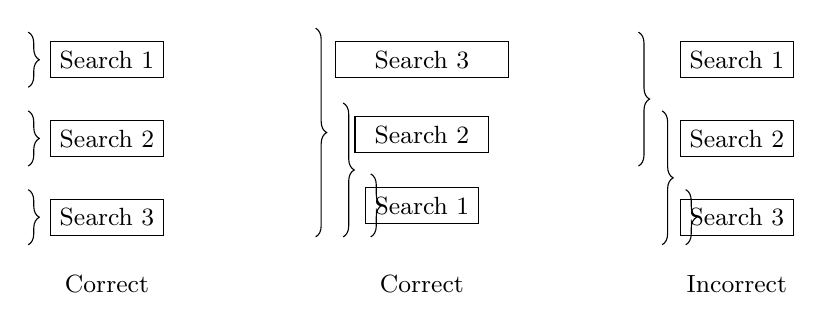
\begin{tikzpicture}[font=\small,
  block/.style={draw,minimum width=1.4cm,minimum height=0.45cm,align=center},
  brace/.style={decorate,decoration={brace,amplitude=4pt}}]
  % Independent searches
  \node[block] (a1) at (0,1.5) {Search 1};
  \node[block] (a2) at (0,0.5) {Search 2};
  \node[block] (a3) at (0,-0.5) {Search 3};
  \draw[brace] (-1.0,1.85) -- (-1.0,1.15);
  \draw[brace] (-1.0,0.85) -- (-1.0,0.15);
  \draw[brace] (-1.0,-0.15) -- (-1.0,-0.85);
  \node at (0,-1.35) {Correct};

  % Nested searches
  \node[block,minimum width=2.2cm] (b3) at (4.0,1.5) {Search 3};
  \node[block,minimum width=1.7cm] (b2) at (4.0,0.55) {Search 2};
  \node[block,minimum width=1.2cm] (b1) at (4.0,-0.35) {Search 1};
  \draw[brace] (2.65,1.9) -- (2.65,-0.75);
  \draw[brace] (3.0,0.95) -- (3.0,-0.75);
  \draw[brace] (3.35,0.05) -- (3.35,-0.75);
  \node at (4.0,-1.35) {Correct};

  % Intersecting searches
  \node[block] (c1) at (8.0,1.5) {Search 1};
  \node[block] (c2) at (8.0,0.5) {Search 2};
  \node[block] (c3) at (8.0,-0.5) {Search 3};
  \draw[brace] (6.75,1.85) -- (6.75,0.15);
  \draw[brace] (7.05,0.85) -- (7.05,-0.85);
  \draw[brace] (7.35,-0.15) -- (7.35,-0.85);
  \node at (8.0,-1.35) {Incorrect};
\end{tikzpicture}

  \caption{Valid multiple-search structures.}
  \label{fig:multiple-search-structures}
\end{figure}

For nested searches, the looping structure can be clarified with dummy segments
whose final condition is such as \texttt{tseg>0}. These segments have zero duration
and do not alter the trajectory, but they provide segment endpoints at which search
objective functions can be evaluated.
